%%
%% Copyright 2007, 2008, 2009 Elsevier Ltd
%%
%% This file is part of the 'Elsarticle Bundle'.
%% ---------------------------------------------
%%
%% It may be distributed under the conditions of the LaTeX Project Public
%% License, either version 1.2 of this license or (at your option) any
%% later version.  The latest version of this license is in
%%    http://www.latex-project.org/lppl.txt
%% and version 1.2 or later is part of all distributions of LaTeX
%% version 1999/12/01 or later.
%%
%% The list of all files belonging to the 'Elsarticle Bundle' is
%% given in the file `manifest.txt'.
%%

%% Template article for Elsevier's document class `elsarticle'
%% with harvard style bibliographic references
%% SP 2008/03/01
%%
%%
%%
%% $Id: elsarticle-template-harv.tex 4 2009-10-24 08:22:58Z rishi $
%%
%%


%% WHAT WE WERE USING \documentclass[final,authoryear,11pt,times]{elsarticle}

%% Use the option review to obtain double line spacing
%% \documentclass[authoryear,preprint,review,12pt]{elsarticle}

%% Use the options 1p,twocolumn; 3p; 3p,twocolumn; 5p; or 5p,twocolumn
%% for a journal layout:
%% \documentclass[final,authoryear,1p,times]{elsarticle}
%%\documentclass[final,authoryear,1p,times,twocolumn]{elsarticle}
%%\documentclass[final,authoryear,3p,times]{elsarticle}
%%\documentclass[final,authoryear,3p,times,twocolumn]{elsarticle}
\documentclass[final,authoryear,5p,times,twocolumn]{elsarticle}

%% if you use PostScript figures in your article
%% use the graphics package for simple commands
%% \usepackage{graphics}
%% or use the graphicx package for more complicated commands
%% \usepackage{graphicx}
%% or use the epsfig package if you prefer to use the old commands
%% \usepackage{epsfig}

%% The amssymb package provides various useful mathematical symbols
\usepackage{amssymb}
\usepackage{amsmath}

%%\usepackage[margin=1.25in]{geometry}


\usepackage{todonotes}
\usepackage{epigraph}
\usepackage{graphicx}
\usepackage{setspace}
\usepackage{hyperref}
\usepackage{soul}
\usepackage{color}
\usepackage{cleveref}
\crefname{section}{�}{��}
\Crefname{section}{�}{��}
\renewcommand{\sectionautorefname}{\S}
\renewcommand{\subsectionautorefname}{\S}
\onehalfspacing

%% The amsthm package provides extended theorem environments
%% \usepackage{amsthm}

%% The lineno packages adds line numbers. Start line numbering with
%% \begin{linenumbers}, end it with \end{linenumbers}. Or switch it on
%% for the whole article with \linenumbers after \end{frontmatter}.
%% \usepackage{lineno}

%% natbib.sty is loaded by default. However, natbib options can be
%% provided with \biboptions{...} command. Following options are
%% valid:

%%   round  -  round parentheses are used (default)
%%   square -  square brackets are used   [option]
%%   curly  -  curly braces are used      {option}
%%   angle  -  angle brackets are used    <option>
%%   semicolon  -  multiple citations separated by semi-colon (default)
%%   colon  - same as semicolon, an earlier confusion
%%   comma  -  separated by comma
%%   authoryear - selects author-year citations (default)
%%   numbers-  selects numerical citations
%%   super  -  numerical citations as superscripts
%%   sort   -  sorts multiple citations according to order in ref. list
%%   sort&compress   -  like sort, but also compresses numerical citations
%%   compress - compresses without sorting
%%   longnamesfirst  -  makes first citation full author list
%%
%% \biboptions{longnamesfirst,comma}

% \biboptions{}

\journal{CS280r, Spring 2017 - Final Project Report, Goldstein and Wihl}

\begin{document}

\begin{frontmatter}

%% Title, authors and addresses

%% use the tnoteref command within \title for footnotes;
%% use the tnotetext command for the associated footnote;
%% use the fnref command within \author or \address for footnotes;
%% use the fntext command for the associated footnote;
%% use the corref command within \author for corresponding author footnotes;
%% use the cortext command for the associated footnote;
%% use the ead command for the email address,
%% and the form \ead[url] for the home page:
%%
%% \title{Title\tnoteref{label1}}
%% \tnotetext[label1]{}
%% \author{Name\corref{cor1}\fnref{label2}}
%% \ead{email address}
%% \ead[url]{home page}
%% \fntext[label2]{}
%% \cortext[cor1]{}
%% \address{Address\fnref{label3}}
%% \fntext[label3]{}

\title{$A \rho \mu o \nu \acute{\iota} \alpha$ (Harmonia): A System for Collaborative Music Composition}

%% use optional labels to link authors explicitly to addresses:
%% \author[label1,label2]{<author name>}
%% \address[label1]{<address>}
%% \address[label2]{<address>}

\author{{\rm Mark Goldstein, David Wihl}\\ Harvard University}
\address{\normalsize\{markgoldstein,davidwihl\}@g.harvard.edu}

\begin{abstract}

Increasing productivity of music composition has many positive benefits. Listeners would appreciate music individually tailored to their emotional needs and context. Composers would be facilitated by greater and more diverse cooperation yielding more innovative music. Composition agents could assist in the generation of repetitive or  experimental musical forms. Therapists can use music as part of a treatment plan  for autism and many other disorders. The system we propose attempts to address these myriad needs  by offering two key innovations: a SharedPlan with versioning to mediate the workflow of a composition for a group of musicians and an algorithmic evaluation of a composition against the intention of the SharedPlan to provide guidance to both human and agent composers.

\end{abstract}

\end{frontmatter}

\section*{Introduction}
\label{sec:introduction}

%\epigraph{It is my design to render it manifest that no one point in its composition is referrible either to accident or intuition -- that the work proceeded, step by step, to its completion with the precision and rigid consequence of a mathematical problem.}{\textit{Edgar Allen Poe, The Philosophy of Composition}}

Music composition is often an individual endeavor, which is counterintuitive when music is mostly performed, improvised, and experienced in a group. Part of this is due to the singular nature of creative expression, but a large part is also due to a dearth of viable tools to enable collaborative efforts between composers. Most modern composition is facilitated through the use of digital audio workstation (DAW) tools, yet composers do not generally have access to tools designed for collaboration, version control, and annotation that are available to software engineering teams.

There are many additional issues that surround collaboration over structured, shared objects such as a music composition. Each composer has a unique artistic vision, and a composer working on one section of a piece may ruin the plans of another working on a later section. It is crucial in such settings that a group specify an artistic goal clearly and communicate their intentions for material as it is added. However, it is also valuable that new ideas can surface as a consequence of the collaborative process, leading to material that could not be created by any one artist. How can composers stay connected with an original goal and also make room for spontaneity?

Collaborative Ideation (CI) investigates the effect of various idea-sharing tactics on the creativity, productivity and scope of individual idea-generating participants. Such techniques may include showing each participant in a pool of brainstormers the collection of all participants' brainstormed ideas. In CI that focuses on the creation of shared objects such as a composition or story by several people, certain interfaces for collaboration, automated idea-sharing mechanisms, and per-participant system feedback may help facilitate group creativity and productivity.

SharedPlans provide a framework to establish and maintain context and metadata about group artistic work. This framework ensures that the collaborative process and ideation stay within reasonably agreed parameters, provides a formalized notion of common beliefs and defines a means of independent instrumentation that the work-in-progress is navigating toward the original intention.

We propose a system that addresses collaborative music composition inspired by tools used for software teamwork, collaborative ideation, and musical structure analysis. This system defines an interface for collaboration over a shared creative artifact, and includes procedures for editing a work-in-progress and receiving algorithmic  feedback about edits. Crucially, the system assists collaborators with the task of staying on track with an \textit{a priori} specified goal for the turnout of the piece, and also provides a framework for communication among collaborators about the intention of edits during collaboration.


In \S \ref{sec:related}~ we examine previous work related to shared intentionality, collaboration and group ideation, intelligent music systems, and modeling the structure of music. In \S \ref{sec:design}~ we describe the details of the overall usage workflow, as well as the individual components of our system. This includes a specification of an automated approach for giving composers feedback on the relevance of their ideas to a specified collaborative goal. We present four use cases for our system in \S \ref{sec:usecases}~, where collaborating composers create music ranging in purpose from casual listening to clinical therapy. In \S \ref{sec:discuss}~ we discuss limitations that we have identified in our system, and a few initial plans for system validation. We discuss potential future work in \S \ref{sec:future}~.

\section{Related Work}
\label{sec:related}

Our work builds on several areas of research related to music, computer science, and creative cognition. First we discuss related work regarding shared intentionality in multi-agent settings. Then we discuss collaborative ideation, both in general and specifically in music. Next we discuss intelligent music systems that facilitate human composition and improvisation, and related work in Music Information Retrieval (MIR). Finally we describe previous work that applies information theory to the analysis of musical structure.

\subsection{Shared Plans}

SharedPlans \citep{grosz1996collaborative, hunsberger1998making} define a robust framework for multi-agent, multi-level collaboration. A SharedPlan consists of a set of intentions, mutual beliefs, constraints, and hierarchies of actions and plans. All of these elements are applicable in this context, although only a subset of the general definition is needed for music composition purposes. 

A SharedPlan is the basic unit of work for a collaborative group in our system. It serves as the container for the initial definition of the intent of the work, the musical score representing the work-in-progress, the revision history, the sub-plans used to communicate between composers, and the final approval given by the user who defined the SharedPlan initially.

Intentions are expressed by a minimum of two criteria: genre and mood. These are algorithmically combined using existing methods (See \S \ref{sec:analysis}~ \nameref{sec:analysis}) to define the approximate representation of the final work.
  
Mutual beliefs are expressed implicitly in the trust of the automated analysis system that powers genre / mood combination, structure evaluation, and edit recommendation. This extends the notion of beliefs in SharedPlans to \hl{a predictable instrumentation of common understanding, simplifying integration of both human and agent composers}. Mutual beliefs are expressed explicitly through sub-goal communication.

There is one complex action and one Full SharedPlan in this scenario: production of a score that meets the intention. Each composer may divide the complex action into a series of sub-actions (See \S \ref{subsec:editActions}~ \nameref{subsec:editActions}). If a composer is unable to complete all actions necessary to achieve the intention, a sub-plan is created stating the Intention-To for a future composer. This is the primary means that composers communicate with each other. We do not define a means of using \textit{recipes} in this context.

We use the term composer in the singular form, however a single composer may work as part of several collaborating humans to produce an edit. Any such informal communication is beyond the scope of our proposal. After collaborating, a single human would execute edits on composition toward the intended goal. For example, a composer may improvise with colleagues to explore several alternatives of a sub-plan. Once a consensus is achieved that the section meets artistic and SharedPlan goals, one composer commits an edit.

\subsection{Collaborative Ideation}
% Collaborative Ideation In General
Collaborative Ideation (CI) improves the productivity of individuals and groups in generating ideas through collaboration. People intend to create related objects (e.g., brainstorm solutions to social problems) and seek either feedback or examples of others' work to enhance their individual process. Collaboration is centered in a shared workspace, physical or virtual, that allows for communication and sharing of ideas. The ideas produced may be for individual use, or ideators may work on shared artifacts such as an essay or piece of art. The dynamics of collaboration may be real-time or not, though increasingly, today's settings are real-time and virtual \footnote{\texttt{https://www.openideo.com/}}\footnote{\texttt{http://www.ideastorm.com/}}\footnote{\texttt{https://www.quirky.com/}} \citep{openinnovation}. A simple CI setting is one where each ideator brainstorms solutions to a problem common to all participants, and each participant can see all other's ideas. The design of intelligent computer systems today aims to facilitate these activities to allow for increased creativity and productivity. 

%IdeaHound
Only a small subset of an idea pool may be relevant and inspiring to a single ideator, and it is overwhelming for each ideator to view all participant's ideas \citep{siangliulue2015toward}. Ideahound \citep{siangliulue2016ideahound} prompts each user to interact with a personal ``whiteboard" where they can cluster their ideas and separate them by semantic distance. A global semantic map is computed by compiling the whiteboards, allowing each ideator to view their work in the context of the entire solution space. IdeaHound recommends diverse suggestions to each ideator, eliminating the cognitive load of idea search. 

When exposed to the work of others, composers may come up with things they would not make on their own.  In our work, CI is made explicit when a composer addresses a sub-plan instantiated by another (See \S \ref{subsec:interComposer}~ \nameref{subsec:interComposer}). Generated objects are structured, rather than unordered collections of ideas, and ideators need to build over each other's ideas rather than only seek inspiration from examples by others. These details present new challenges.

%Soundcloud and Blend
CI has surfaced in the space of online blogs and services designed to share visual art and music. Ideas range from small, unfinished efforts seeking direction to finished pieces seeking critique. Artists improve upon their ideas using large-scale feedback. SoundCloud is a hybrid music streaming service and CI platform. Though music is often presented in finished form, people also post incomplete projects. Artists sometimes share ``stems" to their music, which are individual sound files that feature isolated instrumental tracks, with the intention that others seeking inspiration remix their pieces into new work. 

The Blend platform \footnote{\texttt{https://blend.io}} makes the sharing of source files explicit. By default, artists share their works-in-progress in the format of music production software source files, which allows others to quickly pick up on their work. This setting encourages building on each other's ideas. However, people mostly work toward an ultimately individual direction. What changes when several ideators intend to create a shared piece? In our work, a composition is associated with a specified intent through the duration of its existence. It is up to the composers and the system to keep a piece of music close to its SharedPlan.

\subsection{Computer Facilitated Composition and Improvisation}

% Music Info Retrieval in General
Intelligent Music Systems ranging from composition and improvisation facilitating agents to recommendation systems have a common requirement, to ``understand" music at multiple levels, including low-level acoustic signal, mid-level theoretical constructs such as harmony and rhythm, and high-level level aspects such as mood, genre, and style. For example, a music recommendation system such as Spotify \footnote{\texttt{https://www.spotify.com}} seek to analyze music and extract a measure of relevance for a function such as ``study music". These issues constitute the research area of Music Information Retrieval (MIR).

% ChordRipple
In systems that create music, the interest is to assist human composers, rather than replace them. Perhaps a composer has good ``seeds" ideas, but the system may recommend variations of ideas, or re-orderings of ideas, to make them more conveying. Such system knowledge often comes from large-scale corpus analysis that mines patterns common to a collection of music. ChordRipple \citep{huang2016chordripple} takes as input a progression of musical chords from a composer, and suggests substitutions of intermediate chords that preserve the original semantics of the input while serving to replace conventional choices with more interesting ones. If the composer agrees to make one of the recommended changes, the system assists the composer in interpolating between original and substituted material before and after the initial substitution, resulting in further mixing of human and system generated music. Our system makes suggestions to composers, but it focuses on structural changes rather than material substitutions to support collaboration.

% Magenta and AI Duet
While our current work seeks primarily to assist teams of human composers to enrich and organize their work, we intend to design the system such that intelligent computer agent composers may fully participate without requiring human intervention. Last year, Google Brian launched the Magenta Project for exploring limits of machine creativity \footnote{\texttt{https://magenta.tensorflow.org/welcome-to-magenta}}. Magenta is an integrated environment of software tools and music-related datasets. This year, Magenta released AI Duet \footnote{\texttt{https://aiexperiments.withgoogle.com/ai-duet}}, a computer system that reacts to human improvised gestures. Improvisation is an important part of composition. When a single composer is brainstorming, it may be beneficial to improvise on ideas with an automated agent, much like two musicians iteratively vary and refine their ideas in live rehearsals. In settings where a piece is defined by a specific enough set of guidelines (See \S \ref{subsec:therapy1}), a listener may need music at a certain tempo and with a simple beat. Powerful information retrieval systems may make effective machine composition agents possible. Human composers may be placed at later steps of collaboration to ensure that the piece meets requirements in humanly perceptible ways.
%\nameref{subsec:therapy1})

\subsection{Information Theory and Music Analysis}

% Abdallah, Predictive Information Rate
Our systems relies on the ability to analyze musical structure to support automated feedback for collaborating composers. Recent approaches have represented musical form in the context of listener perception, modeling the attention dynamics of the listener as they experience the toggle of surprise and redundancy. The Information Dynamics Approach \citep{abdallah2012cognitive} uses \textit{predictive information rate}, an entropy-based measurement of how a listener's distribution over future musical events is continually revised as new information is presented.  Our work assumes that musical structure can be effectively summarized by this criteria. We assume that pieces from a particular combination of genres and moods are defined by characteristic balances of surprise and redundancy over time, with peaks of information content communicated by the composer(s) in genre-specific locations. We use the Information Dynamics Approach for automated analysis in our system, which compares a collaborative work-in-progress to the characteristic curves for the genre and mood specified by the work's SharedPlan.

\section{System Design}
\label{sec:design}

After reviewing the workflow of editing a piece of music as part of a team of composers, we describe the details of our system design. The design addresses two aspects of collaborative composition. The first includes the composition interface, the representation of music, the editing capabilities of composers, and the version control system used to track musical revisions. These all focus on issues of communication and coordination in collaboration over a shared artifact. The second aspect of design is the automated music analysis used for giving feedback and suggestions to composers. This facilitates the collaborative composition process by helping composers assess the effect of their edits on the movement of the work-in-progress toward a goal. We discuss how these two system components combine to help composers by providing an interface that makes revisions convenient, modular, and amenable to collaboration.

\subsection{Workflow Overview}

\begin{figure}
	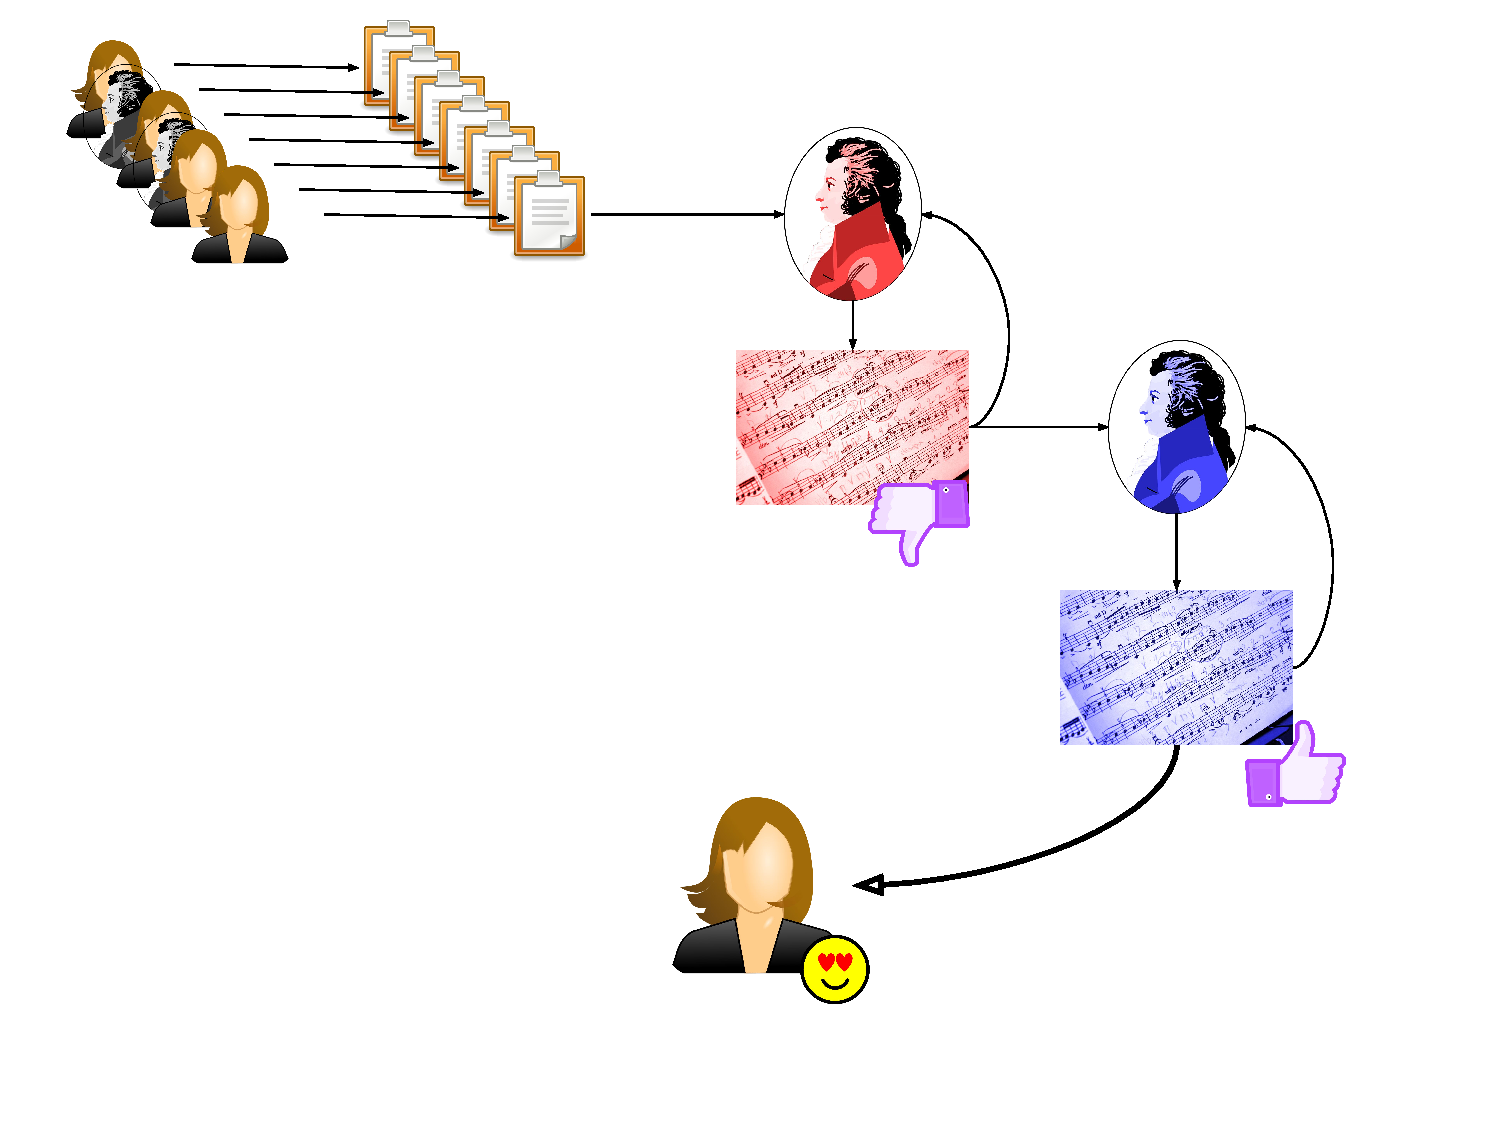
\includegraphics[scale=0.35]{workflow.pdf}
	\caption{Overall workflow: a non-musical user or a composer define a SharedPlan. Composer 1 (\textcolor{red}{red}) starts
	iterating and commits a work-in-progress. Composer 2 (\textcolor{blue}{blue}) continues iterating until the original user is
	satisfied.}
	\label{fig:workflow}
\end{figure}

The generic use case that we consider is that a listener (musician or not) requests a new piece of music of a specified genre and mood, and other related keywords. A new, blank score is associated with a SharedPlan that stores the genre, mood, and optional keywords. The system retrieves MIDI scores for existing related music. The system computes a summary of characteristic musical structure of the retrieved body of work. Composers iteratively add and edit material while receiving system feedback about their edits. The system computes the similarity of the work-in-progress structure to that of characteristic pieces described by the SharedPlan. This feedback helps composers choose which edits are most relevant.  The system also suggests edits, such as to repeat, delete, or the switch the order of blocks of material. 

Composers can follow suggestions or make their own decisions. During this process, composers create sub-goals that describe the intentions of local edits, such that others can pick up on their material and preserve these intentions. Composers collaborate to bring the composition to a state of completion such that it matches the originally specified goals. Composers iterate on the composition until the SharedPlan originator is satisfied. The finished product is a MIDI score for a piece of music.


\subsection{Version Control}

Version control has become an essential part of team-based software development. However, the tools for managing revisions of other creative work, including composition, are nonexistent or limited in comparison. There are two commercial version control systems for music: the aforementioned Blend and Splice.com \footnote{\texttt{https://splice.com/}}. \texttt{git} \citep{torvalds2010git} has been referenced elsewhere \citep{oberholtzer2015computational} as a viable means for musical score version control, especially in the MIDI format. Software based version control systems are excellent for basic operations such as branching, committing and viewing history, but they are lacking several primitives necessary for integration in our proposed workflow. We propose the following additional commands for the workflow:

\noindent \textit{For users and composers}:
\begin{description}
    \item [EditPlan] - create, revise or delete a SharedPlan that includes intentionality and other metadata.
    \item [Approve] - the SharedPlan creator denotes a SharedPlan as satisfactorily executed
    \item [Reject] - the SharedPlan creator denotes a SharedPlan as unsatisfactorily executed
\end{description}

\noindent \textit{For composers only}:
\begin{description}
    \item [Evaluate] - prior to committing a revision, perform an analysis of the current score against intentionality.
    \item [EditSubplan] - create, revise or delete a sub-plan. Creating or editing a sub-plan \hl{would establish the hierarchical context to the SharedPlan. TODO: Not sure what this means}
    \item [Release] - after a commit, mark a work as ready for review by the creator of the sub-plan. This closes the sub-plan. If a plan is rejected, it may be re-opened.
\end{description}

The versioning aspect is particularly relevant in the music context, as intellectual property and originality is often the source of extensive lawsuits. By maintaining version control, an examination of the history would assist in the identification of derivative works and originality of authorship.

\subsection{Communication through SharedPlan and Sub-plans}
\label{subsec:interComposer}
 
When a composition task is created, it exists as a SharedPlan that contains an intent specification, as well as a \texttt{NULL} score. Additional descriptive keywords may be included in the form of tags, like those on YouTube or Soundcloud \footnote{\texttt{https://on.soundcloud.com/creator-guide/tracks}} (\texttt{$\#$USA}, \texttt{$\#$lo-fi}, \texttt{$\#$chill}, \texttt{$\#$electronic}, \texttt{$\#120BPM$}). These tags power an automated comparison between work-in-progress and goal, and helps composers pick edits that may bring a composition closer to a sound characterized by the goal keywords. We assume that an information retrieval system for querying MIDI music scores by keyword exists.

In addition to describing global goals, the SharedPlan also mediates any inter-composer communication that takes place aside from the edits to the composition itself.  A composer may wish to express the intention of a particular edit to justify its presence or to elicit specific future directions for their material. For example, a composer may add a block of music containing an exposed melody, but may want to communicate that another composer should add a harmonic accompaniment to that section. This is done by issuing a sub-goal. Another composer who acts on an open sub-goal \textit{releases} it when they commit their work.

It is ideal for communication to be concise and structured. It may be detrimental to collaborative work for one composer to expect others to read long, unstructured goal descriptions. It may require too high of a cognitive load for the others to carefully read and understand, and the intending composer may not have their ideas respected. We have not yet designed a structured language for describing intent in sub-goals, but we recommend composers to be concise. A structured language may help support automated agent collaborators in the future. This is discussed further in the Therapy case study (See \S \ref{subsec:therapy1}~ \nameref{subsec:therapy1}). 

Intention sharing may help distinguish between two kinds of collaboration issues. The first scenario is where a composer agrees with another composer's intention about an edit, but disagrees with the actual implementation. This may lead to the second composer editing the first composer's material with care to preserve the original sound, or replacing it with something of similar effect. The second scenario is where a composer fundamentally disagrees with the artistic intention of another. An effective SharedPlan communication system may disambiguate these cases.

\begin{figure}
	\centering
	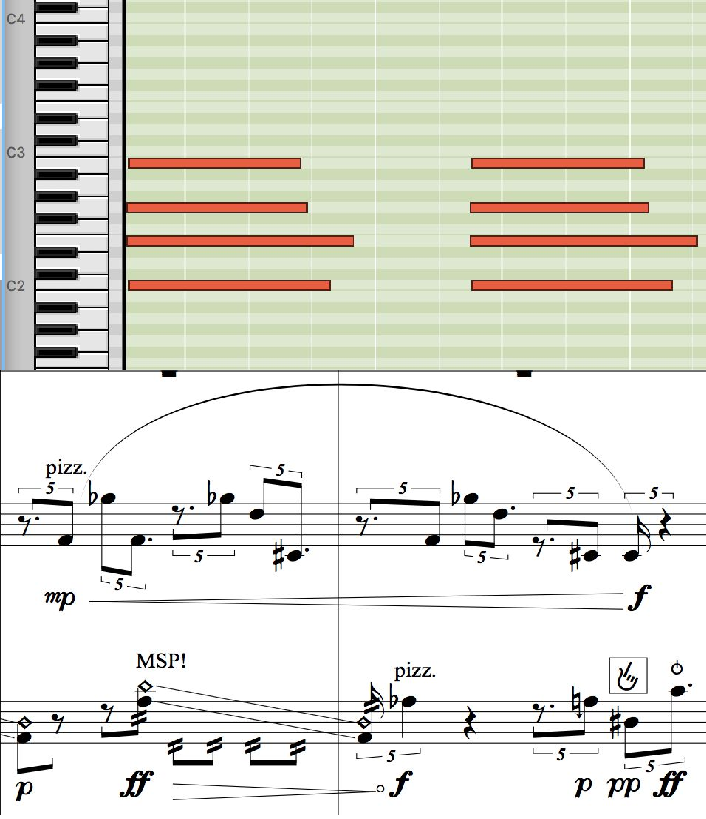
\includegraphics[scale=0.5]{midi.pdf}
	\caption{Music represented by MIDI (top) and MusicXML (bottom)}
	\label{fig:midi}
\end{figure}

\subsection{MIDI and Edit Actions}
\label{subsec:editActions}

Our system represents music in MIDI format. MIDI is a protocol for communicating discrete information about the pitch, duration, and dynamics of individual notes. A musical work is described by specifying the vertical arrangement of individual notes as chords and their horizontal arrangement over time. Additionally, there is a General MIDI Sound bank that maps integers to specific electronic instrument sounds. For example, one can specify that this MIDI part is meant to be played by sound $0$, grand piano or Ocarina, sound $80$. Most familiar software for music notation and music production build user interfaces on top of a basic MIDI file editor. Through the use of additional metadata, composers are able to segment MIDI files into separate segments. For example, a piece may be subdivided into several sections. Segmentation may represent intentions about musical form, for example one may segment part of a composition into an exposition and a development section. 

During an interaction with the system, a composer is able to change a composition by editing the MIDI in several low-level or high-level ways. Composers can add a new block of material, edit an existing block, remove an existing block, swap the order of two blocks, merge two blocks, or split a block into two. At each iteration of editing, the system suggests an option that may bring the work in progress closer to what is specified by the SharedPlan. This is primarily of the form of ``move block A after block B?" (See Section on Automatic Evaluation). The final product of collaboration is a MIDI file that represents the pitches, rhythms, and dynamics of musical events, as well as a collection of metadata that concisely states additional information, such as tempo and instrumentation. 

\begin{table}
    \begin{tabular}{|l|l|}
    	\hline
    	\textbf{Action} & \textbf{Description} \\
    	\hline
    	\textit{Insert,Delete,Replace} & Add, remove or replace a block \\
    	\textit{Move} & Rearrange order of a block \\
    	\textit{Split, Merge} & Divide or combine a block \\
    	\hline
    \end{tabular}
	\caption{Summary of Atomic Edit Actions on Score}
\end{table}

The piece can be produced as an electronic piece of music by importing the MIDI into any music production software, specifying which MIDI track should be played by which sound or synthetic instrument, and exporting a sound file. If desired, composers may take additional actions on that finished work that are external to the system, such as produce the piece of music with live musicians or extended software instruments, but this is beyond our scope, which is mainly to facilitate collaboration during the composition process.

\subsection{Design Failure Modes}

There are multiple potential failure circumstances of the proposed design:

\begin{description}
\item[Failure to compose] No composer may elect to work on a given SharedPlan.
\item[Failure to satisfy] The creator of the original SharedPlan may never approve or reject the produced work, leaving it in an undefined state.
\item[Sub-plan not released]A sub-plan may be defined but no composer ever completes the sub-plan so the work stays in an incomplete state.
\item[Evaluation not converging] The evaluation process may continue to offer suggestions that are rejected by the composer. Note that the evaluation process only makes recommendations but is not a gatekeeper for the composer to release. However, if the Evaluation mechanism repeatedly gives undesired or unhelpful suggestions, composers will cease future use.
\item[Failure to Evaluate] there may not be sufficient training data for a given genre / mood combination so the Evaluation may fail to provide sufficiently useful recommendations.
\end{description}

Failures result in a specific SharedPlan not advancing, but none of these failures affect other SharedPlans in the system.

\section{User Interface}

There are three aspects to the user interface: for non-musical users, for composers performing workflow and for composers actively editing the musical score.

\subsection{SharedPlan Workflow User Interface}

There are three possible commands in this context: \textbf{EditPlan} (including create/edit/delete), \textbf{Approve, Reject}. Since the user may not have any musical background, this user interface must be accessible to as large a population as possible. Ideally, this would be a simple looking, reactive web-based interface that would work equally well on mobile devices as well as desktops. Music apps such as Spotify may wish to integrate this functionality so a web-based API must also be accessible.

For an unsophisticated user, \textbf{Approve} and \textbf{Reject} may be considered implicit. If the user listens to the composition past a certain point, such as 80\% of the total length of the work, it may be deemed implicitly approved. Similarly, if the user advances to another song within the first 20\% of piece time, the composition is implicitly rejected. Implicit rejection does not provide any causal reason for the rejection, so trial and error analogous to reinforcement learning must be used to discover the hidden reasons why a work was implicitly rejected. Other user actions (such as stopping all music in the middle of play) do not provide enough signal to determine implicit actions so the work's acceptance status remains unknown.

\subsection{Sub-plan Workflow User Interface}

The market reality is the most modern composers use an existing Digital Audio Workstation (DAW) such as Ableton or LogicPro. Rather than replacing the composer's primary user interface, integration should be performed within the menu system of the most common DAWs. There are only two commands required in this context: \textbf{EditSubplan} (including create/edit/delete) and \textbf{Release}. 

\subsection{Composer Edit / Evaluation User Interface}

This is the most complex and demanding user interface as it requires the highest degree of interactivity. Rather than re-implementing the multitude of music editing features of a mature DAW, integration to existing DAWs is again preferable over creating a \textit{de novo} user interface. The most novel aspect would be the integration of the evaluation to the editing task. Ideally the evaluation result would decorate and annotate the score; enabling the composer to address results of the evaluation while remaining in a known editing context, analogous to seeing and resolving comments in Microsoft Word or a Google Doc.

\section{Automated Analysis of Musical Structure}
\label{sec:analysis}

Harmonia facilitates collaborative composition in two ways. First, the interface as a whole, including the revision system and the shared metadata associated with each composition, helps with practical aspects of communication and coordination. Second, the analysis system lets composers know how close their work-in-progress is to their goal, as measured by similarity to characteristic pieces relevant to their goal. The analysis system also suggests structural edits such as swapping the order of existing material, or deleting material, that could further improve the piece. In this section, we describe the automated analysis of musical structure that is used by our system. Crucial to our system, our computational approach models the structure of a piece of music in relation to the expected trajectory of surprise and redundancy that a listener experiences. Our work follows directly from The Information Dynamics Approach. \citep{abdallah2012cognitive} We first discuss the nature of the musical analysis used in our system, and then discuss how this method supports goal checking and suggested musical edits.

\subsection{Entropy of Musical Events and Divergence}
 
Let $X$ be a discrete random variable that takes on values from the set $\mathcal{X}$. For example, $X$ may represent the next chord that a listener hears in a piece of music. The event $X=x$ indicates that the listener heard $X$ take on a specific value $x$. Let $p_X(x) = p(x)$ denote the probability that $X$ will take on value $x$, \textit{before} the listener hears the chord, as estimated by a distribution that the listener brings with them from prior musical experiences, as well as from what they have heard in the piece so far. $-\log\ p(x)$ then corresponds to the \textit{surprise} of the event, because the more the listener expects the event (higher $p(x)$), the lower the surprise, where the log is taken for convenience (it is monotonic in the $p(x)$). Since $X$ represents the event that the listener is about to hear, we can represent the expected surprise of $X$ averaged over all possible values as:
 
 $$ H(X) = - \sum_{x \in \mathcal{X}} p(x) \log p(x)$$
 
\noindent which corresponds to the Entropy of $X$, $H(X)$. Intuitively, this means that the listener does not know what the next event will be (e.g. which chord will be played next), but from context (from their state of listening as represented by their current distribution over future events), they expect a certain extent of surprise from the next event in general.

Because we choose to represent musical structure in terms of the surprise dynamics of the listener, it is necessary to describe the way in which the listener's distribution over future events changes as they hear present events. In the running example, by hearing $X=``A\flat^{\Delta7}"$ in the present, how does their distribution over future events differ from how it was before they heard that chord. The Kullback-Leibler Divergence of one distribution from another captures this notion of distance between distributions. Avoiding subscripting $X$ with timesteps, let  $X'$ be the revised distribution over the next event \textit{after} hearing $X=x$ in the context of the existing distribution.

$$ D_{KL}(X^{\prime}\textrm{ }|| \textrm{ } X) =  \sum_{x \in \mathcal{X}} p_{X^{\prime}}(x) log\frac{p_{X^{\prime}}(x) }{p_{X}(x)}$$

\noindent This is read as ``the divergence from X' of X", and is the average over the ratio of point-wise log probabilities between the two distributions, weighted by $p_{X'}(x)$. For an accessible yet informative discussion of the significance of entropy as a measure of information and KL Divergence  \footnote{Another interpretation of entropy is the average number of bits required to send a message from a distribution $p$ under an optimal variable-length coding scheme. The KL Divergence of $q$ from $p$ is the increase in the average bits per message when one communicates items from $p$ using a code optimized for $q$. This is the difference between the cross entropy $H(p,q)$ and entropy $H(p)$.}, see Christopher Olah's post on Visual Information Theory \footnote{\texttt{http://colah.github.io/posts/2015-09-Visual-Information}}. This divergence describes the amount of revision to a listener's distribution over the future that happens as they hear each event. Let this be called the \textit{predictive information} of the event $X=x$ as the listener hears it. When a surprising event occurs and causes the listener to drastically revise their distribution (i.e. this same event will be less surprising in the future), the event had high predicative information. On the other hand, if thirty strikes of the same chord have just happened, hearing a thirty-first articulation does not communicate much predictive information. Our system measures the predicative information \textit{rate} (PIR) over the duration of the piece (or work-in-progress), and uses this trajectory of this rate to summarize the structure of a piece of music as it is expected to be perceived by the listener. In the running example, entropy and divergence are discussed with respect to chord sequences heard by the listener, and their expectation over next chords in context. In even a simple piece of music, the listener tracks multiple such parameters and their interactions: evolving harmony, rhythm, timbre, and more (See \S \ref{sec:future}~ \nameref{sec:future}).


\subsection{Current Design: Analyze, Suggest, and Edit}

Harmonia uses PIR to calculate the proximity of a musical work in progress to a characteristic piece from the category specified by the SharedPlan. Using these measures, the system gives feedback to a composer with respect to the composer's editing decisions, and provides suggestions that may bring a piece closer to the goal. It is this analysis and suggestion loop, along with interaction with the SharedPlan metadata, that characterize the main experience for an individual composer. This experience is further enriched by the fact that each time the composer enters the feedback loop, the piece and aspects of SharedPlan may have changed by other composers.

We assume that music information retrieval systems exist to facilitate calculating PIR on sample pieces of music queried by genre, mood, and other metadata keywords (HipHop, Chill, Slow, Study)\footnote{\texttt{https://www.youtube.com/watch?v=xrbrQhpvn8E}}. Because we currently analyze MIDI representation of music, this retrieval is done on a corpus of MIDI and score representations of music rather than audio recordings. We calculate the PIR for the most popular $\boldsymbol{\beta}\%$ of pieces matching a specified query (where $\boldsymbol{\beta}$  is a parameter to be specified), and average the PIR curves to create a ``characteristic curve" that represents the typical structure of a piece of music fitting the criteria. \hl{HOW IS THIS AVERAGE CREATED?}

Comparing the characteristic curve with the PIR curve of the work in progress, our system can estimate a notion of distance from the musical goal specified in the SharedPlan. Let the difference be denoted as $\Delta$. This comparison supports several important features of our system. First, not considering any edit suggestions made by our system, a composer may simply see whether their latest edit brings the piece of music closer to (lower $\Delta$) or further from (higher $\Delta$) the SharedPlan. \hl{HOW IS THIS DIFFERENCE CALCULATED?}

Composers may prefer to go with edits that decrease $\Delta$, or may choose to stick with their edit even if it increases $\Delta$. Reasons for going with a ``worsening" action include choosing to lay down material that further edits will re-contextualize, whether by the same composer or by others. In this case, it is important for a composer to commit their intention for the new edit (as concise text) into the SharedPlan metadata as a sub-plan. Future work involves specifying this format more explicitly, so that an automated agent may be able to act in response to this intention. It is also the case that unstructured, non-concise description of intentions by one composer may be difficult or overwhelming for another composer to deal with.

Also using these PIR scores, our system may give actionable edit suggestions. As specified in \S \ref{subsec:editActions}~ \nameref{subsec:editActions}, a composer may edit a piece by adding a new block of material (of any length), edit an existing block, remove a block, swap two blocks, merge two blocks into one, or split one block into two. Excluding adding or editing blocks because this requires intelligent automated composition, and excluding splitting and joining blocks because this does not actually change any musical material or it's ordering, the system may recommend repeating or deleting any existing block, or swapping any pair of existing blocks. Because for any work-in-progress of reasonable length there is a tractably enumerable set of such choices, the system can just try each choice of deleting, repeating, and swapping, and suggest to the user the choice the minimizes $\Delta$. This choice may be the ``make no change" choice at a given iteration, because the best thing to do may be to add more material before considering such actions.

\section{Use Cases}
\label{sec:usecases}

\subsection{Use Case 1: Individual User, Individual Composer}

Our first use case considers the following scenario: a listener who may be a non-musician would like a new piece of music, perhaps for a very specific function such as study music. We consider the case that the listener specifies a new project defined by a mood and genre. In this simple case, we consider a single composer who iterates over the piece with assistance from our system until the requester is satisfied.
%implicitly satisfied \hl{[TODO: What do you mean implicitly?]} by listening to at least 80\% of the piece.

\subsection{Use Case 2: Multiple Composers}

\begin{figure}
	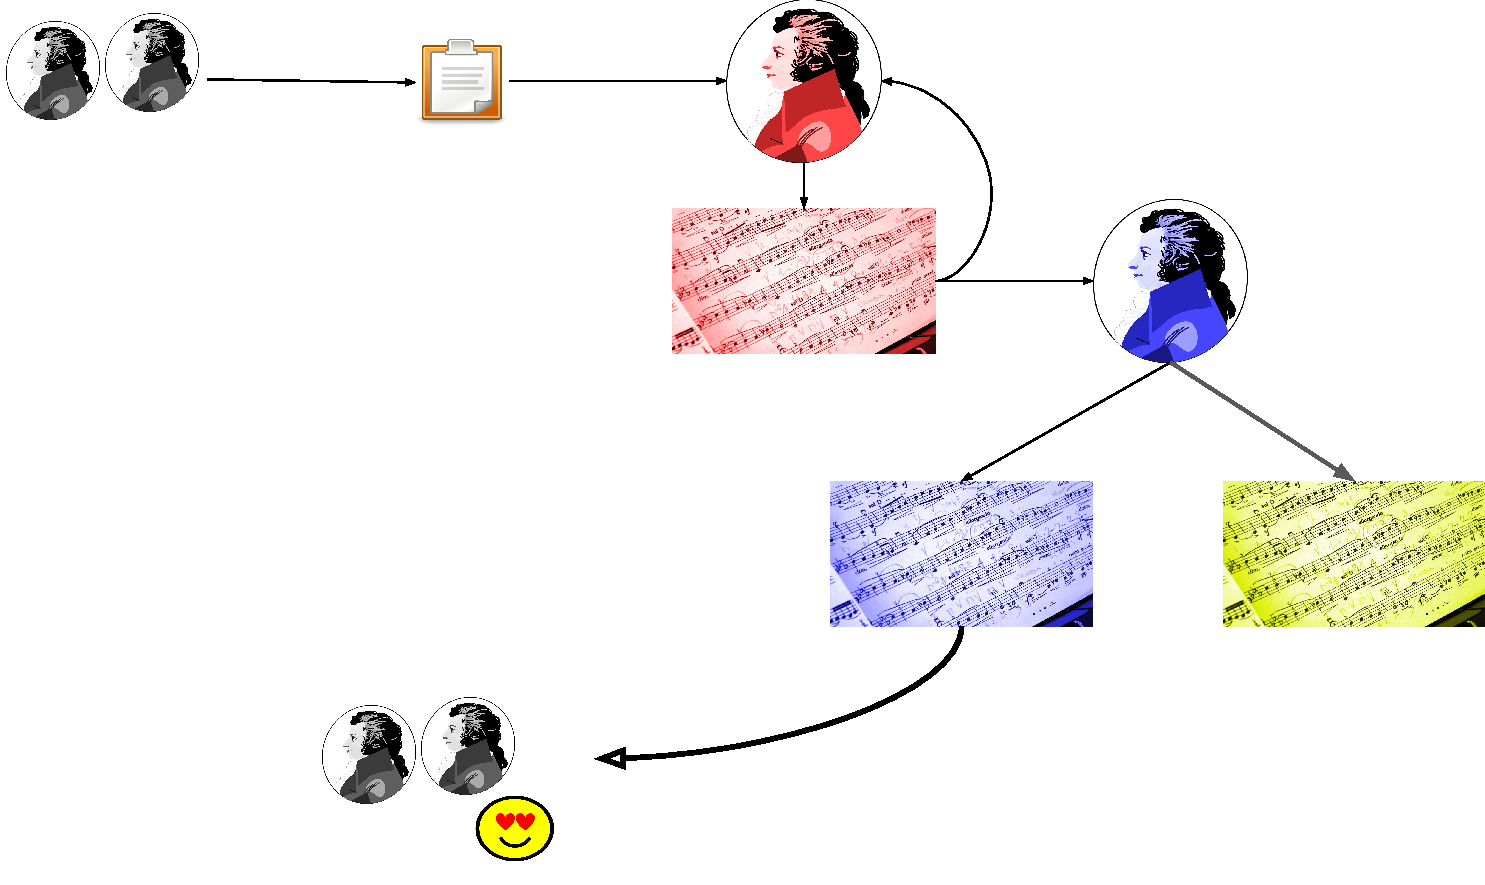
\includegraphics[scale=0.35]{multicomposer.pdf}
	\caption{Use Case 2: Multiple composers define a SharedPlan. Composer 1 (\textcolor{red}{red}) starts
	iterating, commits a work-in-progress and defines a sub-plan. Composer 2 (\textcolor{blue}{blue}) retrieves the sub-plan and continues iterating until the original composers are
	satisfied. Composer 2 maintains a separate branch for personal investigation.}
	\label{fig:multicomposer}
\end{figure}

Our second use case considers multiple composers who create a SharedPlan together, and then collaboratively create the specified piece. During the process, a composer may wish to take the piece into a new direction that doesn't correspond to the SharedPlan. They are able to create a new branch of revision history to experiment on before attempting to re-integrate material with the original group or creating a new SharedPlan with the material. On the main branch, composers issue sub-plans to give each other the opportunity to give someone else an opportunity to complete their idea when they are stuck. Even an insufficient attempt by another composer to release the sub-plan may inspire the issuer. See \S \ref{subsec:eval}~ for a discussion of composer-system interaction success criteria.

\subsection{Use Case 3: Therapist with Agent \& Human Composers}
\label{subsec:therapy1}

\begin{figure}
	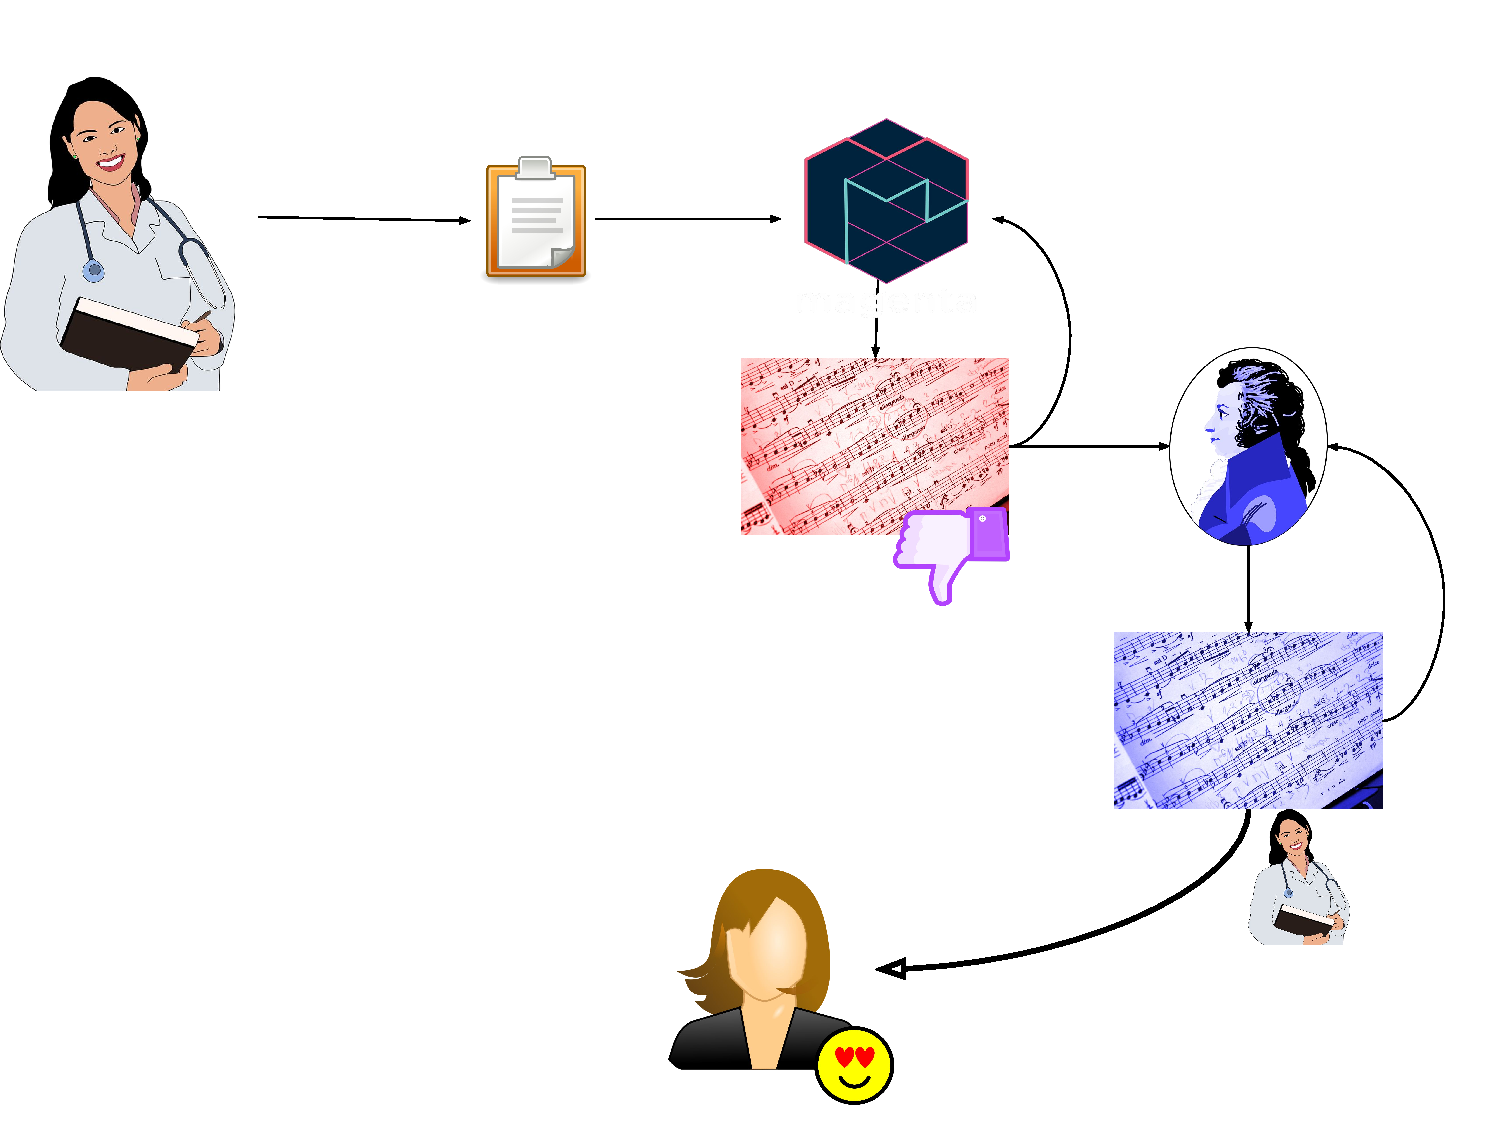
\includegraphics[scale=0.35]{clinical.pdf}
	\caption{Use Case 3: A clinician defines a SharedPlan with more complex metadata for therapeutic use. An agent performs the initial composition which consists of the bulk of the work.	A human composer reviews the work and makes minor adjustments. The clinician approves the work and provides the result to the patient for treatment.}
	\label{fig:clinical}
\end{figure}

Our third case considers the situation where a music therapist treats his or her patients using newly composed music, specific to a given patient's needs. Music therapy is used in many contexts including children and adults with mood disorders (e.g. depression and PTSD), developmental disorders (e.g. autism and ADHD), and neurological conditions (e.g. dementia) \citep{hole2015music}. This SharedPlan may have a more highly refined specification than music for casual listening, such as a specific tempo or special therapeutic timbres (sound qualities). 

Due to high volume of personal treatment plans, the initial SharedPlan worked on by an agent, which performs the bulk of the composition. Consider an agent in the reinforcement learning setting, exploring the space of musical edits while in a feedback loop with the automated evaluation system. The agent's composition is then reviewed by a human who may make only small modifications to make the music more warm or less mechanical. The clinician makes the final approval and then provides the music to the patient for treatment.

\subsection{Use Case 4: Pseudo Music Therapist}

For those who do not have access to a music therapist, Harmonia can be used as a platform to assist patients in achieving certain goals and outcomes, such as creating a song that will express sadness or grief, or to express acceptance and hope for the future \citep{dalton2006grief}. The recommendations generated by the evaluation process can assist a non-musically trained composer to create reasonably sounding music for emotional expression. The act of creative composition is itself therapeutic employing various regions in the brain, including the region responsible for autobiographical memory in the case of improvisation. \citep{hilliard2001effects,bensimon2008drumming,limb2008neural,carr2012group} 

\section{Discussion}
\label{sec:discuss}

\subsection{Evaluation Methodology}
\label{subsec:eval}
 
We intend to validate our system with several studies on small groups of composers that specify a musical goal and collaborate on a piece of music facilitated by our system (Use Case 2). We also intend to validate our system for Use Case 1, in which a non-musician requester seeks for their musical desires to be addressed. The Therapy use cases should be included in studies once these two less-complex cases are assessed. Testing will include the validation of several system aspects:

\begin{enumerate}

\item Do composers understand and benefit from system feedback? If the composer proposes edits $A$ and $B$, and the system scores $B$ higher than $A$, which does the composer pick? What percentage of scores do composers take agreeable actions on? For system-suggested edits, what percentage of suggestions do composers accept?

\item Do composers feel that communication through sub-plans is efficient for collaborating on ideas requiring the work of several composers?

\item Do composers and requesters feel as if finished pieces respect the SharedPlan? 

\end{enumerate}

To address the point 1, we can compare composer experience using 1a) our revision and metadata system without automated analysis 1b) system with analysis for score feedback to composer-specified edits, but no system-suggested edits (reorderings, repeats, deletes). 1c) system with analysis for both score feedback to composer-specified edits and system suggestions. To address the point 2, we should explore other methods of inter-composer communication in place of the sub-plan issue/release procedure. Two approaches are 2a) traditional email to complement version-controlled music with no sub-plan options 2b) additional text documents to describe the equivalent of sub-plans but external to the SharedPlan and in longer form, committed along with the SharedPlan + musical score. Point 3 will come from discussion with the requester and composers.

The percentage of edit suggestion that each user takes does not only describe the success of the system's suggestions, but also the personality of each composer: are they generally open to suggestions or do they tend to stick with their own ideas? This will help to not blame the system for poor performance when dealing with a composer that tends not to take suggestions in general. Aspects of a composer's collaboration profile may also be collected orthogonally to system usage through simple collaboration games (to be designed).

Several obstacles remain to setup the studies. This involves implementation of the system, including information retrieval aspects that are beyond the scope of our work. Because compositions may take some time to work on, these studies will not be very quick. We may try to design smaller-scale composition tasks for these purposes.

\subsection{Enhancing or Stifling Creativity}

The question arises whether algorithmic evaluation of a composition is a potential means of stifling music creativity. Is it possible that a corpus based evaluation will nudge composers into making music that resembles existing work rather free creative expression? Firstly, the evaluation can be ignored by composer -- there is purposefully no gatekeeper function of the Evaluation, it is purely advisory. Secondly, by using an entropy-based evaluation, the composer now has a means of determining the originality of the creation. The Evaluation could be further enhanced to show the composer that the work-in-progress resembles certain existing works too closely, avoiding potential future intellectual property infringement. No composer can possibly know all existing work in the corpus. A composer can now have an independent measure of the originality of the new work, which will encourage greater creativity.

\subsection{Limitations}
\label{subsec:limitations}

There are several limitations in this proposal that are inherent in the design. This is purposeful, as addressing these limitations may result in undo expansion of intent, scope, or problem tractability. Nevertheless, it is important to be explicit about known limitations:

\textit{No explicit support for improvisation.} The collaborative design is inspired from software engineering teamwork, which is a solitary activity. Unlike software, in music very fruitful results may occur in real-time improvisation by several musicians. The design does not preclude improvisation but does not account for it either. There may be interesting paths to explore, discovered during improvisation that would not be captured by this design. A composer would have to create separate branches and record improvisation sections in each branch. The design does not account for partial interchange between branches.

\textit{Information Theory.} Although we have presented the way in which PIR may be calculated over a single musical parameter such as chord progressions or rhythms, composers create many complex relationships across parameters. In the Con Espressione Manifesto, Widmer cites several theorists from the 1950s that were working on modeling music as information \citep{widmer2016getting}. Among them, \cite {cohen1962information} demanded 1) a theory of interactions for multiple streams of musical information, for example, to explain how rhythmic information may make harmonic events more or less certain. 2) a theory for multiple levels of hierarchy coming at once from a single stream of musical information. Rhythms constitute a local time feel but also accelerate a piece toward new sections. These are still complicated aspects of information today. The first point requires a generalization of mutual information to multiple random variables, which has been met with confusion through several coexistent approaches \citep{van2011two}. To our knowledge, the second point has not yet been explored.

\textit{Model may not generalize.} While we are confident that SharedPlans, software revision control, and algorithmic evaluation are applicable to music composition, it is uncertain that the overall framework can be generalized to other domains. Version control for visual artwork seems promising, but simple text-based revision may not support editing capabilities for rich-enough representations of visual art in an intuitive or useful way.  Algorithmic evaluation of intent may be more difficult to design for a painting. Musical form, as treated by our system, is experienced at an information-general level also applicable to a story, movie, or play, but which is limited to sequential forms. The static experience of a painting is less related and may require a different set of domain-specific criteria for capturing intent. To this end, generalizable techniques for automated analysis that bypass the necessity to encode domain-specific information are desirable, and may be approached with today's Deep Learning techniques (See \S \ref{sec:future}~ \nameref{sec:future}).

\textit{Representation is MIDI, not recorded acoustic signal. Vocals are not supported.} MIDI is far easier to generate and maintain under version control, but has two limitations. The first is that many interesting sounds such as vocals and other samples of recorded sound cannot be expressed in the current design. MIDI placeholders may be made for these sounds, such that someone substitutes them into the piece post-collaboration, but collaboration over these sounds themselves is not supported. Given this setting of \textit{written}, rather than \textit{performed} music, the second limitation is that MIDI encodes only a subset of written musical expression. MusicXML is another text-based format that is more flexible than MIDI, while still being amenable to revision control (See Figure 2). It allows musicians to visually communicate performance techniques (e.g. pizzicato, slur, sul ponticello) but would complicate SharedPlan communication protocol and automated analysis.

\textit{Corpus based shared beliefs may not be robust.} One of the key assumptions is that genre / mood permutations generate a reasonable representation of the intent of the music. This representation is corpus-based. This assumption presumes that genre and mood classification solutions exist, particularly for information retrieval procedures and that the representation is robust enough for the evaluation function to provide useful guidance. Since this has not been built and validated, the certainty of this assumption remains a source of further investigation.



\section {Future Work}
\label{sec:future}

Harmonia is intended to serve as a base platform for multiple aspects of musical creativity, while maintaining a sufficiently modular design to evolve. Specifically, the area of creative agents is undergoing rapid evolution. Providing a framework to ensure shared intentionality, artistic consistency and collaboration with humans should provide further acceleration. Multi-agent online improvisation such as AI Duet is another ripe area for exploration both for artistic purposes as well as for `call and response' treatment of autism and other disorders. 

The current automated analysis system is based on hand-crafted entropic measures specific to music information. Given the rapid advance of Recurrent Neural Nets in natural language understanding and other sequential data streams, further investigation is warranted for applying Deep Learning to musical evaluation. In general, a Deep Learning approach to \textit{analysis} of music \citep{deepgenre} is a huge (and exciting) obstacle in the training of automated, musically interactive agents, which could have roles in our system. If Harmonia were used by a large set of users, the resulting listening dataset would provide important training data for applying Reinforcement Learning and other methods to further enhance agent composition. A larger dataset would also be of significant benefit to music therapists who could share empirical data on effective treatments tailored to specific demographic and psychographic profiles.

As mentioned previously, there are significant limits when using MIDI for musical expression. Incorporating more complex musical encoding formats such as recorded audio, or at least MusicXML, would allow for greater range of expression but would complicate analysis. Adding vocals is an interesting challenge. Given recent developments in speech generation, is it possible to further the idea to vocals?\footnote{\texttt{https://lyrebird.ai/}} Can a neural net be programmed to `sing' like Alicia Keys?  Commercial applications of Harmonia include the aforementioned intellectual property similarity evaluation. The evaluation module may also incorporate commercial goals such as potential popularity \citep{phampredicting}.

\section*{Conclusion}
  
Our proposal contributes two novel areas of collaborative music composition. First, we present a workflow incorporating SharedPlans with explicit intentionality, sub-plans, Collaborative Ideation, revision control and automated agents. Second, we present algorithmic evaluation of the composition against intention, to ensure that both human and agent composers cooperate in reaching the shared objective. These contributions extend the state of the art, beyond the ideation of SoundCloud and the revision control without intentionality of Blend. As discussed in \S \ref{sec:future}~ \nameref{sec:future}, we see this initial proposal as a start of several interesting areas to explore leading to improved creativity, diversity and applicability of music composition as a tool for composers, music therapists and listener pleasure.
 
 
\section*{Acknowledgements}

We are honored to be part of Professor Grosz's final class. We deeply appreciate the guidance that she and Peter Krafft have provided all semester. We wish them all the best in their future endeavors and SharedPlans.

Special thanks to \href{https://www.psychologytoday.com/experts/david-m-greenberg-phd}{Dr. David Greenberg}, who provided important insights and suggestions regarding the application of Harmonia for music therapy, to composers Daniel Pencer and Ariel Herbert-Voss, whose discussions about the proposed user interface of our system were highly valuable, and to Pao Siangliulue, for the discussions about composer communication and open innovation platforms.


%%%%%%%%% OPEN ITEMS %%%%%%%%%%%%%%%%%

%------------------ MARK TODOs --------------------------------

%1) Music analysis section: resolve two open questions

%3) Reduce Related Work

%------------------ David TODOs --------------------------------

%1) Consolidate and de-dup intro, workflow and use cases

%------------------ GENERAL TODOs --------------------------------

%1) Fix the bibliography and in-text citations

%2) Another pass or two at spelling and grammar, text revision, clean read through

%3) Ensure that body of report stays within 8-10 page limit



% NOTE: Replaced the class-provided elsarticle-num-names with elsarticle-num-names-alpha
%       to enable sorting of references.
% See https://tex.stackexchange.com/questions/297283/order-references-alphabetically-with-elsarticle-num-names-bst
% and https://github.com/erelsgl/erelsgl.github.io/blob/master/papers/elsarticle-num-names-alpha.bst
%
% To revert to the prior bibliographystyle, change the following line back to:
%             \bibliographystyle{elsarticle-num-names}

\bibliographystyle{elsarticle-num-names-alpha}
\bibliography{harmonia-bib}


\end{document}

%\subsection{Citations}

% MUST ADD ENTRY TO BIB FILE FIRST

%Here are two examples of how to cite a paper properly:
%\begin{itemize}
%	\item \citet{bernstein2000complexity} shows that ... 
%	\item Prior work has shown that ... \citep{bernstein2000complexity}.
%\end{itemize}

%%  \citet{key}  ==>>  Jones et al. (1990)
%%  \citep{key}  ==>>  (Jones et al., 1990)




%% The Appendices part is started with the command \appendix;
%% appendix sections are then done as normal sections
%% \appendix

%% \section{}
%% \label{}

%% References
%%
%% Following citation commands can be used in the body text:
%%
%%  \citet{key}  ==>>  Jones et al. (1990)
%%  \citep{key}  ==>>  (Jones et al., 1990)
%%
%% Multiple citations as normal:
%% \citep{key1,key2}         ==>> (Jones et al., 1990; Smith, 1989)
%%                            or  (Jones et al., 1990, 1991)
%%                            or  (Jones et al., 1990a,b)
%% \cite{key} is the equivalent of \citet{key} in author-year mode
%%
%% Full author lists may be forced with \citet* or \citep*, e.g.
%%   \citep*{key}            ==>> (Jones, Baker, and Williams, 1990)
%%
%% Optional notes as:
%%   \citep[chap. 2]{key}    ==>> (Jones et al., 1990, chap. 2)
%%   \citep[e.g.,][]{key}    ==>> (e.g., Jones et al., 1990)
%%   \citep[see][pg. 34]{key}==>> (see Jones et al., 1990, pg. 34)
%%  (Note: in standard LaTeX, only one note is allowed, after the ref.
%%   Here, one note is like the standard, two make pre- and post-notes.)
%%
%%   \citealt{key}          ==>> Jones et al. 1990
%%   \citealt*{key}         ==>> Jones, Baker, and Williams 1990
%%   \citealp{key}          ==>> Jones et al., 1990
%%   \citealp*{key}         ==>> Jones, Baker, and Williams, 1990
%%
%% Additional citation possibilities
%%   \citeauthor{key}       ==>> Jones et al.
%%   \citeauthor*{key}      ==>> Jones, Baker, and Williams
%%   \citeyear{key}         ==>> 1990
%%   \citeyearpar{key}      ==>> (1990)
%%   \citetext{priv. comm.} ==>> (priv. comm.)
%%   \citenum{key}          ==>> 11 [non-superscripted]
%% Note: full author lists depends on whether the bib style supports them;
%%       if not, the abbreviated list is printed even when full requested.
%%
%% For names like della Robbia at the start of a sentence, use
%%   \Citet{dRob98}         ==>> Della Robbia (1998)
%%   \Citep{dRob98}         ==>> (Della Robbia, 1998)
%%   \Citeauthor{dRob98}    ==>> Della Robbia


%% References with bibTeX database:

